\documentclass{beamer}

\usepackage{beamerthemesplit}
\usetheme{Singapore} %Copenhagen}
%\usecolortheme{whale}

\usepackage[T2A]{fontenc}
\usepackage[utf8]{inputenc}
\usepackage[russian]{babel}


\usepackage{textcomp}
\usepackage{amssymb,amsmath}
%\usepackage{animate}
%\usepackage{longtable}
\usepackage{xcolor}

%\usepackage{pstricks}

\newcounter{N}

\usebackgroundtemplate{
\includegraphics[width=\paperwidth]{../img/background.png}}

%% Форматирование окружения itemize
%\usepackage{ragged2e}
%\let\olditem\item
%\renewcommand\item{\olditem\justifying}


\title[]{Аффинный ортогональный тензор}

\author[]{к.ф.-м.н. {\em Верещагин Антон Сергеевич}\\
%Институт теоретической и прикладной механики\\ им.~С.~А.~Христиановича СО РАН\\
\bigskip
\bigskip
\bigskip
\bf Лекция 2\\
\bigskip
}

\newtheorem{dfn}{Определение}  
\newtheorem{theorems}{Теорема}  

\newcommand{\Rn}{\mathrm{R}^n}
\newcommand{\Sm}{\mathrm{S}^m}
\newcommand{\Ql}{\mathrm{Q}^l}

\newcommand{\Rd}[1]{\mathbb{R}^{#1}}
\newcommand{\Vn}{\mathrm{V}^n}

\newcommand{\oper}[1]{{\bf #1}}
\newcommand{\basis}[1]{\vec{\bf #1}}
\newcommand{\dt}[1]{\frac{d #1}{dt}}
\newcommand{\dtds}[1]{\displaystyle\frac{d #1}{dt}}
\newcommand{\ds}[1]{\frac{d #1}{ds}}
\newcommand{\dsds}[1]{\displaystyle\frac{d #1}{ds}}
\newcommand{\dsd}[1]{\frac{d^2 #1}{ds^2}}
\newcommand{\pdt}[1]{\frac{\partial #1}{\partial t}}
\newcommand{\pds}[1]{\frac{\partial #1}{\partial s}}
\newcommand{\pdx}[1]{\frac{\partial #1}{\partial x}}
\newcommand{\pdy}[1]{\frac{\partial #1}{\partial y}}
\newcommand{\pdz}[1]{\frac{\partial #1}{\partial z}}
\newcommand{\pdxds}[1]{\displaystyle\frac{\partial #1}{\partial x}}
\newcommand{\pdyds}[1]{\displaystyle\frac{\partial #1}{\partial y}}
\newcommand{\pdzds}[1]{\displaystyle\frac{\partial #1}{\partial z}}
\newcommand{\pdn}[1]{\frac{\partial #1}{\partial n}}
\newcommand{\grad}[1]{\operatorname{grad} #1}
\newcommand{\gradv}[1]{\basis{i}\pdx{#1}+\basis{j}\pdy{#1}+\basis{k}\pdz{#1}}
\newcommand{\gradvds}[1]{\basis{i}\pdxds{#1}+\basis{j}\pdyds{#1}+\basis{k}\pdzds{#1}}

\newcommand{\pd}[2]{\frac{\partial #1}{\partial #2}}

\newcommand{\pdxt}[1]{\frac{\partial^2 #1}{\partial x^2}}
\newcommand{\pdyt}[1]{\frac{\partial^2 #1}{\partial y^2}}
\newcommand{\pdzt}[1]{\frac{\partial^2 #1}{\partial z^2}}


\newcommand{\dv}[1]{\operatorname{div}\vec{#1}}
\newcommand{\dvdef}[1]{\pdx{#1_x}+\pdy{#1_y}+\pdz{#1_z}}
\newcommand{\dvdefds}[1]{\pdxds{#1_x}+\pdyds{#1_y}+\pdzds{#1_z}}
\newcommand{\dvwv}[1]{\operatorname{div} #1}
\newcommand{\rot}[1]{\operatorname{rot}\vec{#1}}
\newcommand{\rotpr}[2]{\operatorname{rot}_{#1}\vec{#2}}
\newcommand{\rotwv}[1]{\operatorname{rot} #1}

\newcommand{\lapl}[1]{\pdxt{#1}+\pdyt{#1}+\pdzt{#1}}

\newcommand{\argq}{(q_1,q_2,q_3)}
\newcommand{\argx}{(x,y,z)}
\newcommand{\tensor}[1]{\boldsymbol{#1}}


\begin{document}

\frame{\titlepage}


\frame{
\frametitle{Аннотация}
\parbox{\textwidth}{
Аффинный ортогональный тензор второго ранга. Диада. Сопряженный тензор. Симметричные и антисимметричные тензоры. Теоремы о разложении тензора. Скалярное и векторное умножение тензора на вектор. Скалярное произведение тензоров.
}
}



\frame{
\frametitle{Аффинный ортогональный вектор}



\begin{columns}
\begin{column}{0.4\textwidth}
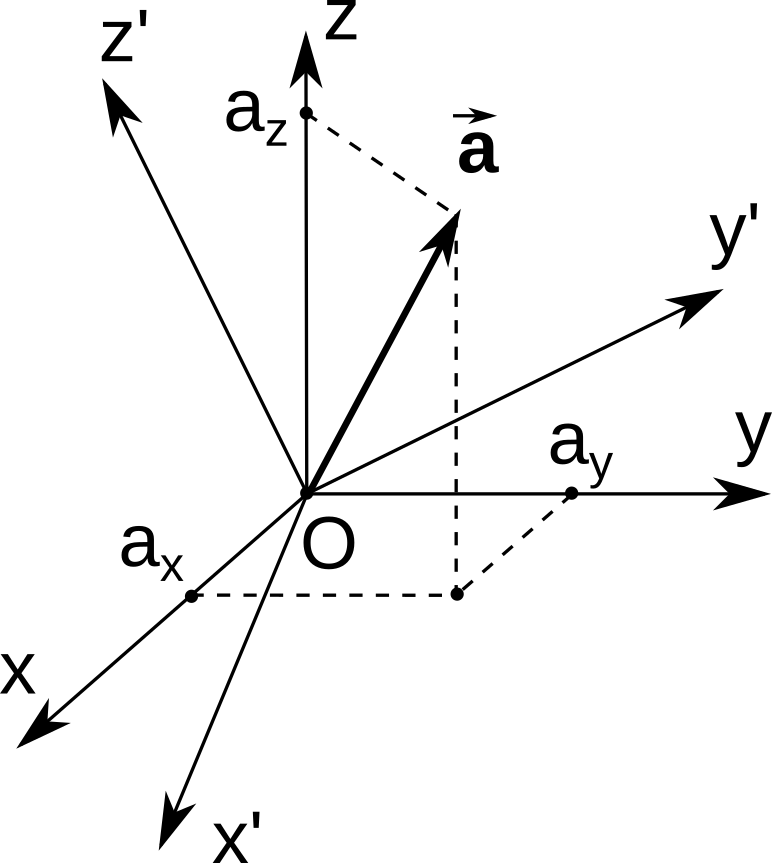
\includegraphics[width=\textwidth]{../img/vector.png}
\end{column} \pause 
\begin{column}{0.6\textwidth}
\parbox{\textwidth}{
Пусть в некоторой ортогональной прямолинейной системе координат $Oxyz$
\[ 
\vec{a}=\basis{i}a_x+\basis{j}a_y+\basis{k}a_z.
\] \pause 
Тогда в другой ортогональной прямолинейной системе координат $Ox'y'z'$ вектор будет иметь координаты:
}
\end{column}
\end{columns}



\begin{eqnarray*}
a_{x'} & = & a_x \cos (x,x')+a_y \cos (y,x')+a_z \cos (z,x'),\\ \pause 
a_{y'} & = & a_x \cos (x,y')+a_y \cos (y,y')+a_z \cos (z,y'),\\ \pause 
a_{z'} & = & a_x \cos (x,z')+a_y \cos (y,z')+a_z \cos (z,z').
\end{eqnarray*}
}

\frame{
\frametitle{Аффинный ортогональный вектор}

\begin{dfn}
\parbox{\textwidth}{
Если для прямолинейной ортогональной системы координат $Oxyz$ имеется совокупность трех величин $a_x$, $a_y$, $a_z$, преобразующихся по вышеуказанным формулам в величины $a_{x'}$, $a_{y'}$, $a_{z'}$, в другой ортогональной прямолинейной системе координат $Ox'y'z'$,  \pause то совокупность этих величин определяет \alert{аффинный ортогональный вектор} $\vec{a}$. Скалярные величины $a_x$, $a_y$, $a_z$ называются составляющими (компонентами) вектора $ \vec{a} $ по осям $Ox$, $Oy$, $Oz$.
}
\end{dfn}
}

\frame{
\frametitle{Аффинный ортогональный тензор второго ранга}

\begin{dfn}
\parbox{\textwidth}{
Если для прямолинейной ортогональной системы координат $Oxyz$ имеется совокупность трех векторов $\vec{p}_{x}$, $\vec{p}_{y}$, $\vec{p}_{z}$, преобразующихся по формулам в величины $\vec{p}_{x'}$, $\vec{p}_{y'}$, $\vec{p}_{z'}$, в другой системе координат $Ox'y'z'$:
\begin{eqnarray*}
\vec{p}_{x'} & = & \vec{p}_x \cos (x,x')+\vec{p}_y \cos (y,x')+\vec{p}_z \cos (z,x'),\\
\vec{p}_{y'} & = & \vec{p}_x \cos (x,y')+\vec{p}_y \cos (y,y')+\vec{p}_z \cos (z,y'),\\
\vec{p}_{z'} & = & \vec{p}_x \cos (x,z')+\vec{p}_y \cos (y,z')+\vec{p}_z \cos (z,z'),
\end{eqnarray*} \pause 
то совокупность этих величин определяет \alert{аффинный ортогональный тензор второго ранга}. Векторы $\vec{p}_{x}$, $\vec{p}_{y}$, $\vec{p}_{z}$ называются составляющими (компонентами) тензора $ \Pi $ по осям $Ox$, $Oy$, $Oz$.
}
\end{dfn}




}


\frame{
\frametitle{Матричное представление тензора}
\parbox{\textwidth}{

Будем обозначать 
\[ 
\tensor{\Pi}=\basis{i}\vec{p}_x+\basis{j}\vec{p}_y+\basis{k}\vec{p}_z.
\] \pause 
%\medskip
Таким образом, тензор представляет собой набор из 9 компонент:
\[
\tensor{\Pi}=
\begin{pmatrix}
p_{xx} & p_{xy} & p_{xz} \\
p_{yx} & p_{yy} & p_{yz} \\
p_{zx} & p_{zy} & p_{zz}
\end{pmatrix} \pause 
\begin{array}{cc}
\leftarrow & \vec{p}_x = p_{xx}\basis{i} + p_{xy}\basis{j} + p_{xz}\basis{k}\\
\leftarrow & \vec{p}_y = p_{yx}\basis{i} + p_{yy}\basis{j} + p_{yz}\basis{k}\\
\leftarrow& \vec{p}_z = p_{zx}\basis{i} + p_{zy}\basis{j} + p_{zz}\basis{k} 
\end{array}
\] \pause 
%где $$, $$, $$

В дальнейшем:
\begin{itemize}
\item вместо координат $x$, $y$,$z$ будем писать $x_1$, $x_2$, $x_3$;
\item базисные векторы будем обозначать $\basis{i}_1$, $\basis{i}_2$, $\basis{i}_3$;
\item компоненты тензора будем нумеровать, т.е. $p_{ij}$ ($i,j=\overline{1,3}$).
\end{itemize} 
}
}

\frame{
\frametitle{Преобразование ортогональных систем координат}

\parbox{\textwidth}{
Пусть задано некоторое преобразование одной ортогональной прямолинейной системы координат в другую с помощью матрицы преобразования, т.е. заданы направляющие косинусы единичных векторов новых базисных векторов $\alpha_{ik}=\cos(x_i,x'_k)$:
\begin{columns}
\begin{column}{0.4\textwidth}
\begin{equation*}
Q=\begin{pmatrix}
\alpha_{11} & \alpha_{12} & \alpha_{13} \\
\alpha_{21} & \alpha_{22} & \alpha_{23} \\
\alpha_{31} & \alpha_{32} & \alpha_{33}
\end{pmatrix},
\end{equation*} \pause 
\end{column}
\begin{column}{0.6\textwidth}
\[
\left\{
\begin{array}{ll}
\sum\limits_{i=1}^3\alpha_{is}^2=1 & (s=\overline{1,3}),\\
\sum\limits_{i=1}^3\alpha_{is}\alpha_{ik}=0 & (s,k=\overline{1,3}; s \neq k).
\end{array}
\right.
\]
\end{column}
\end{columns} \pause 

\bigskip
Таким образом, $Q$ -- ортогональная матрица, т.к.
\[
Q^{-1}=Q^{\rm t}.
\]
%Для компонент справедливы следующие равенства
}


}


\frame{
\frametitle{Компоненты тензора в штрихованной системе координат}

\parbox{\textwidth}{
Компоненты вектора $\vec{a}$ и тензора $\tensor{\Pi}$ в новой штрихованной системе координат $a'_1$, $a'_2$, $a'_3$ и $\vec{p'}_{1}$, $\vec{p'}_{2}$, $\vec{p'}_{3}$ имеют вид:
\[
a'_{k}=a_{x'_k}=\sum\limits_{i=1}^3\alpha_{ki}a_{x_i}, \quad 
\vec{p'}_k=\vec{p}_{x'_k}=\sum\limits_{i=1}^3\alpha_{ki}\vec{p}_{x_i} \quad (k=\overline{1,3}).
\] \pause 

%Выясним при этом как меняются скалярные компоненты тензора $\Pi$.

Проекция вектора $ \vec{p}_{x'_k} $ на ось $x'_l$:
$
(\vec{p}_{x'_k})_{x'_l}=\displaystyle\sum\limits_{r=1}^3\alpha_{kr} (\vec{p}_{x_r})_{x'_l}
$. \pause 

Из определения аффинного вектора:
$
(\vec{p}_{x_r})_{x'_l}=\displaystyle\sum\limits_{s=1}^3\alpha_{ls} \vec{p}_{x_rx_s}
$. \pause 

\medskip
Подставим последнее равенство в предпоследнее:
\begin{center}
$
p_{x'_kx'_l}=\displaystyle\sum\limits_{r=1}^3\sum\limits_{s=1}^3\alpha_{kr}\alpha_{ls}p_{x_rx_s}
$
или 
$
p'_{kl}=\displaystyle\sum\limits_{r=1}^3\sum\limits_{s=1}^3\alpha_{kr}\alpha_{ls}p_{rs}. 
$
\end{center}
}
}

\frame{
\frametitle{Определение тензора (альтернативное)}
\begin{dfn}[альтернативное]
\parbox{\textwidth}{
Если для каждой прямолинейной прямоугольной системы координат  $Ox_1x_2x_3$ имеется совокупность девяти величин $p_{kl}$, преобразующихся в величины $p'_{kl}$ в новой системе координат $Ox'_1x'_2x'_3$ по формуле:
\[
p'_{kl}=\displaystyle\sum\limits_{r=1}^3\sum\limits_{s=1}^3\alpha_{kr}\alpha_{ls}p_{rs},
\]
то совокупность этих величин определяет \alert{аффинный ортогональный тензор второго ранга} $\tensor{\Pi}$ в пространстве трех измерений.
}
\end{dfn}


}

\frame{
\frametitle{Альтернативная запись тензора}
\parbox{\textwidth}{
Записанную в новых обозначения формулу для разложения векторов 
\[ 
\vec{p}_k=\sum\limits_{l=1}^3\vec{i}_l p_{kl}, \quad (k=1,2,3)
\] \pause 
подставим в равенство, определяющее тензор, и получим условную запись
\[ 
\tensor{\Pi}=\sum\limits_{k=1}^3\sum\limits_{l=1}^3\vec{i}_k\vec{i}_lp_{kl}.
\]
}
}

\frame{
\frametitle{Единичный тензор}
Пусть
\[
\tensor{I}=\basis{i}_1\basis{i}_1+\basis{i}_2\basis{i}_2+\basis{i}_3\basis{i}_3.
\]


Тензор $\tensor{I}$ называется \alert{единичным} тензором. \pause
\[
\tensor{I}=
\begin{pmatrix}
1 & 0 & 0 \\
0 & 1 & 0 \\
0 & 0 & 1
\end{pmatrix} \pause 
\begin{array}{cc}
\leftarrow & \vec{p}_1 = \basis{i}_1\\
\leftarrow & \vec{p}_2 = \basis{i}_2\\
\leftarrow & \vec{p}_3 = \basis{i}_3 
\end{array}\pause
\quad\quad
p_{rs}=\delta_{rs}=
\left\{
\begin{array}{c}
1, r=s, \\
0, r\neq s.
\end{array}
\right.
\] \pause 

В альтернативной системе координат
\[
p'_{kl}= \pause \sum\limits_{r=1}^3\sum\limits_{s=1}^3\alpha_{kr}\alpha_{ls}p_{rs}= \pause 
\sum\limits_{r=1}^3\alpha_{kr}\alpha_{lr}= \pause 
\delta_{kl}. 
\]\pause

\parbox{\textwidth}{
Тензор $\tensor{I}$ имеет одни и те же компоненты в любой ортогональной системе координат.

}
}

\frame{
\frametitle{Диада}

\begin{dfn}
\parbox{\textwidth}{
Пусть $\vec{a}=\basis{i}_1a_1+\basis{i}_2a_2+\basis{i}_3a_3$ и $\vec{b}=\basis{i}_1b_1+\basis{i}_2b_2+\basis{i}_3b_3$, \pause тогда \alert{диадным} или \alert{тензорными произведением} векторов $\vec{a}$ и $\vec{b}$ называется тензор, определяемый следующим соотношением: \pause 
\[
\vec{a}\otimes\vec{b}=
\vec{a}\vec{b}= \pause 
\begin{pmatrix}
a_1b_1 & a_1b_2 & a_1b_3 \\
a_2b_1 & a_2b_2 & a_2b_3 \\
a_3b_1 & a_3b_2 & a_3b_3 
\end{pmatrix}
\]


}
\end{dfn}

}

\frame{
\frametitle{Корректность определения диады }
При переходе к новой системе координат $Ox'_1x'_2x'_3$ компоненты этих векторов преобразуются по формулам: 
\[
a'_k=\sum\limits_{r=1}^3\alpha_{kr}a_r, \quad b'_l=\sum\limits_{s=1}^3\alpha_{ls}b_s \quad (k,l=1,2,3).
\] \pause 

Перемножив оба эти равенства, получим
\[
a'_kb'_l=\sum\limits_{r=1}^3\sum\limits_{s=1}^3\alpha_{ks}\alpha_{ls}a_rb_s.
\]
следовательно приведенное выражение является тензором по определению (альтернативному).


}

\frame{
\frametitle{Сопряженный тензор}

\begin{dfn}
\parbox{\textwidth}{
Тензор $\tensor{\Pi}_c$ называется \alert{сопряженным} к тензору $\tensor{\Pi}$, если компоненты его получены транспонированием компонент тензора $\tensor{\Pi}$.
}
\end{dfn} \pause 

\begin{exampleblock}{Сопряжение диады}

\[
(\vec{a}\vec{b})_c= \pause 
\begin{pmatrix}
a_1b_1 & a_1b_2 & a_1b_3 \\
a_2b_1 & a_2b_2 & a_2b_3 \\
a_3b_1 & a_3b_2 & a_3b_3 
\end{pmatrix}_c= \pause 
\begin{pmatrix}
a_1b_1 & a_2b_1 & a_3b_1 \\
a_1b_2 & a_2b_2 & a_3b_2 \\
a_1b_3 & a_2b_3 & a_3b_3 
\end{pmatrix}= \pause 
\vec{b}\vec{a}. \pause 
\]

\end{exampleblock}
Таким образом, $(\vec{a}\vec{b})_c=\vec{b}\vec{a}$.

}

\frame{
\frametitle{Сумма тензоров}
\begin{dfn}
\parbox{\textwidth}{
\alert{Суммой} тензоров $\tensor{A}$ и $\tensor{B}$ называется тензор $\tensor{C}$, компоненты которого равны сумме компонент тензоров $\tensor{A}$ и $\tensor{B}$. Пишут $\tensor{C}=\tensor{A}+\tensor{B}$.
}
\end{dfn} \pause 

\medskip
\parbox{\textwidth}{
Используя альтернативное определение легко показать, что определение суммы корректно, т.е. $\tensor{C}$ является тензором.
}
}

\frame{
\frametitle{Симметричный тензор}

\begin{dfn}
\parbox{\textwidth}{
Тензор $\tensor{S}$ называется \alert{симметричным}, если $\tensor{S}_c=\tensor{S}$.
}
\end{dfn} \pause 

\begin{exampleblock}{Покомпонентная запись симметричного тензора}
\parbox{\textwidth}{
\[
\tensor{S}=
\begin{pmatrix}
p_{11} & p_{12} & p_{13} \\
p_{12} & p_{22} & p_{23} \\
p_{13} & p_{23} & p_{33}
\end{pmatrix}
\] \pause 
Симметричный тензор определяется 6 компонентами.
}
\end{exampleblock}

}


\frame{
\frametitle{Антисимметричный тензор}
\begin{dfn}
\parbox{\textwidth}{
Тензор $\tensor{A}$ называется \alert{антисимметричным}, если $\tensor{A}_c=-\tensor{A}$.
}
\end{dfn} \pause 

\begin{exampleblock}{Покомпонентная запись антисимметричного тензора}
\parbox{\textwidth}{
Введем вектор $\vec{\omega}=\vec{i}_1\omega_1+\vec{i}_2\omega_2+\vec{i}_3\omega_3$. \pause 
Тогда 
\[
A=\basis{i}_1\vec{p}_1+\basis{i}_2\vec{p}_2+\basis{i}_3\vec{p}_3= \pause 
\begin{pmatrix}
0 & -\omega_3 & \omega_2 \\
\omega_3 & 0 & -\omega_1 \\
-\omega_2 & \omega_1& 0 
\end{pmatrix},
\] \pause 
где $\vec{p}_1  =  -\omega_3\basis{i}_2+\omega_2\basis{i}_3=\basis{i}_1\times\vec{\omega}$,  \pause 
$\vec{p}_2  =  \omega_3\basis{i}_1-\omega_1\basis{i}_3=\basis{i}_2\times\vec{\omega}$,  \pause 
$\vec{p}_3 = -\omega_2\basis{i}_1+\omega_1\basis{i}_2=\basis{i}_3\times\vec{\omega}$. \pause 

\medskip
Таким образом, $A=\basis{i}_1(\basis{i}_1\times\vec{\omega})+\basis{i}_2(\basis{i}_2\times\vec{\omega})+\basis{i}_3(\basis{i}_3\times\vec{\omega})$.  \pause 

\medskip
Антисимметричный тензор задается 3 компонентами.

}
\end{exampleblock}

}

\frame{
\frametitle{Теорема о разложении тензора}
\begin{theorems}
\normalfont
\parbox{\textwidth}{
Всякий тензор можно разложить, и притом единственным образом, на сумму симметричного и антисимметричного тензора.
}
\end{theorems} \pause 

\begin{proof}
\parbox{\textwidth}{
Пусть задан тензор $\tensor{\Pi}$.  \pause Легко убедиться, что
\[
\tensor{\Pi}=\tensor{S}+\tensor{A},
\] 
где
$\tensor{S}=\displaystyle\frac{\tensor{\Pi}+\tensor{\Pi}_c}{2}$ -- симметричный, а $\tensor{A}=\displaystyle\frac{\tensor{\Pi}-\tensor{\Pi}_c}{2}$ -- антисимметричный тензоры. Действительно,
\[
\begin{array}{l}
\tensor{S}_c= \pause 
\left(\displaystyle\frac{\tensor{\Pi}+\tensor{\Pi}_c}{2}\right)_c= \pause 
\displaystyle\frac{\tensor{\Pi}_c+(\tensor{\Pi}_c)_c}{2}= \pause 
\displaystyle\frac{\tensor{\Pi}+\tensor{\Pi}_c}{2}= \pause 
\tensor{S},\\
\tensor{A}_c= \pause 
\left(\displaystyle\frac{\tensor{\Pi}-\tensor{\Pi}_c}{2}\right)_c= \pause 
\displaystyle\frac{\tensor{\Pi}_c-(\tensor{\Pi}_c)_c}{2}= \pause 
-\displaystyle\frac{\tensor{\Pi}-\tensor{\Pi}_c}{2}= \pause 
-\tensor{A}.
\end{array}
\]

}
\end{proof}
}

\frame{
	\frametitle{Теорема о разложении тензора}
	\begin{theorems}
		\normalfont
		\parbox{\textwidth}{
			Всякий тензор можно разложить в сумму трёх диад, такое разложение не единственно.
		}
	\end{theorems} \pause 
	
	\begin{proof}
		\parbox{\textwidth}{
			Пусть задан тензор $\tensor{\Pi}$. Легко убедиться, что
			\[ 
			\tensor{\Pi}=\basis{i}\vec{p}_x+\basis{j}\vec{p}_y+\basis{k}\vec{p}_z,
			\]
			где $\basis{i}$, $\basis{j}$, $\basis{k}$ -- базисные векторы пространства $R^3$; $\vec{p}_x$, $\vec{p}_y$, $\vec{p}_z$~--~ компоненты тензора в указанном базисе.
		}
	\end{proof}
}

\frame{
	\frametitle{Скалярное и векторное умножение тензора на вектор}
	
	\begin{dfn}
		\parbox{\textwidth}{
			Под \alert{скалярным произведением тензора} $ \tensor{\Pi} = \vec{i}_1\vec{p}_1+\vec{i}_2\vec{p}_2+\vec{i}_3\vec{p}_3$ \alert{на вектор} $ \vec{a}=\vec{i}_1a_1+\vec{i}_2a_2+\vec{i}_3a_3 $ \alert{справа} будем понимать вектор $ \vec{a'}'$:
			\[ 
			\vec{a'}=\tensor{\Pi}\cdot\vec{a}=\vec{i}_1(\vec{p}_1\cdot\vec{a})+\vec{i}_2(\vec{p}_2\cdot\vec{a})+\vec{i}_3(\vec{p}_3\cdot\vec{a}).
			\]
			%\[
			%=\vec{i}_1(p_{11}a_1+p_{12}a_2+p_{13}a_3)+\vec{i}_2(p_{21}a_1+p_{22}a_2+p_{23}a_3)+\vec{i}_3(p_{31}a_1+p_{32}a_2+p_{33}a_3).
			%\]
		}
	\end{dfn}
	\pause 
	
	\begin{dfn}
		\parbox{\textwidth}{
			Под \alert{скалярным произведением вектора} $ \vec{a} $ \alert{на тензор} $ \tensor{\Pi} $ \alert{слева} понимается вектор $ \vec{a''} $:
			\[ 
			\vec{a''}=\vec{a}\cdot\tensor{\Pi}=(\vec{a}\cdot\vec{i}_1)\vec{p}_1+(\vec{a}\cdot\vec{i}_2)\vec{p}_2+(\vec{a}\cdot\vec{i}_3)\vec{p}_3=
			\]
			\[ 
			=a_1\vec{p}_1+a_2\vec{p}_2+a_3\vec{p}_3.
			\]
		}
	\end{dfn}
}

\frame{
	\frametitle{Диада (повтор)}
	
	\begin{dfn}
		\parbox{\textwidth}{
			Пусть $\vec{a}=\basis{i}_1a_1+\basis{i}_2a_2+\basis{i}_3a_3$ и $\vec{b}=\basis{i}_1b_1+\basis{i}_2b_2+\basis{i}_3b_3$, тогда \alert{диадным} или \alert{тензорными произведением} векторов $\vec{a}$ и $\vec{b}$ называется тензор, определяемый следующим соотношением: 
			\[
			\vec{a}\otimes\vec{b}=
			\vec{a}\vec{b}= 
			\begin{pmatrix}
			a_1b_1 & a_1b_2 & a_1b_3 \\
			a_2b_1 & a_2b_2 & a_2b_3 \\
			a_3b_1 & a_3b_2 & a_3b_3 
			\end{pmatrix}=
			\basis{i}_1(a_1\vec{b})+\basis{i}_2(a_2\vec{b})+\basis{i}_3(a_3\vec{b}).
			\]
		}
	\end{dfn} \pause 
	
	\begin{exampleblock}{Линейность диады по каждому аргументу}
		\[
		(\vec{a}+\vec{b})\vec{c} = \vec{a}\vec{c}+ \vec{b}\vec{c}.
		\]
		\[
		\vec{c}(\vec{a}+\vec{b}) = \vec{c}\vec{a}+ \vec{c}\vec{b}.
		\]
		
	\end{exampleblock}
	
}


\frame{
	\frametitle{Скалярное произведение диады на вектор}
	
	Пусть $\vec{a}$, $\vec{b}$, $\vec{c}$ -- вектора.
	
	\[ 
	(\vec{b}\vec{c})\cdot\vec{a}= \pause 
	(\basis{i}_1b_1\vec{c}+\basis{i}_2b_2\vec{c}+\basis{i}_3b_3\vec{c})\cdot\vec{a}= \pause 
	\basis{i}_1b_1(\vec{c}\cdot\vec{a})+\basis{i}_2b_2(\vec{c}\cdot\vec{a})+\basis{i}_3b_3(\vec{c}\cdot\vec{a})= \pause 
	\]
	\[
	=
	(\basis{i}_1b_1+\basis{i}_2b_2+\basis{i}_3b_3)(\vec{c}\cdot\vec{a})= \pause 
	\vec{b}(\vec{c}\cdot\vec{a}).
	\]
	
	\medskip
	\[ 
	\vec{a}\cdot(\vec{b}\vec{c})= \pause 
	\vec{a}\cdot(\basis{i}_1b_1\vec{c}+\basis{i}_2b_2\vec{c}+\basis{i}_3b_3\vec{c})= \pause 
	a_1b_1 \vec{c} + a_2b_2 \vec{c} + a_3b_3 \vec{c}= \pause 
	\]
	\[
	=
	(a_1b_1 + a_2b_2 + a_3b_3) \vec{c}= \pause 
	(\vec{a}\cdot\vec{b})\vec{c}.
	\]
}

\frame{
	\frametitle{Векторное произведение тензора на вектор}
	
	\begin{dfn}
		\parbox{\textwidth}{
			Под \alert{векторным произведением тензора} $ \tensor{\Pi} $ \alert{на вектор} $\vec{a}$ \alert{справа} понимается новый тензор $ \tensor{\Pi'} $, вычисленный по формуле:
			\[ 
			\tensor{\Pi'}=\tensor{\Pi}\times\vec{a}=\vec{i}_1(\vec{p}_1\times\vec{a})+\vec{i}_2(\vec{p}_2\times\vec{a})+\vec{i}_3(\vec{p}_3\times\vec{a}).
			\]
		}
	\end{dfn} \pause 
	
	\begin{dfn}
		\parbox{\textwidth}{
			Под \alert{векторным произведением вектора} $\vec{a}$ \alert{на тензор} $ \tensor{\Pi} $ \alert{слева} понимается новый тензор $ \tensor{\Pi''} $, вычисленный по формуле:
			\[ 
			\tensor{\Pi''}=\vec{a}\times\Pi=(\vec{a}\times\vec{i}_1)\vec{p}_1+(\vec{a}\times\vec{i}_2)\vec{p}_2+(\vec{a}\times\vec{i}_3)\vec{p}_3.
			\]
		}
	\end{dfn} \pause 
}

\frame{
	\frametitle{Векторное произведение диады на вектор}
	
	\[ 
	(\vec{b}\vec{c})\times\vec{a}= \pause 
	(\basis{i}_1b_1\vec{c}+\basis{i}_2b_2\vec{c}+\basis{i}_3b_3\vec{c})\times\vec{a}= \pause 
	\]
	\[
	=
	\basis{i}_1b_1(\vec{c}\times\vec{a})+\basis{i}_2b_2(\vec{c}\times\vec{a})+\basis{i}_3b_3(\vec{c}\times\vec{a})= \pause 
	\vec{b}(\vec{c}\times\vec{a}).
	\] \pause 
	
	\medskip
	\[ 
	\vec{a}\times(\vec{b}\vec{c})= \pause 
	\vec{a}\times(\basis{i}_1b_1\vec{c}+\basis{i}_2b_2\vec{c}+\basis{i}_3b_3\vec{c})= \pause 
	\]
	\[
	=
	(a\times\basis{i}_1) (b_1 \vec{c}) + (a\times\basis{i}_2) (b_2 \vec{c}) + (a\times\basis{i}_3) (b_3 \vec{c})= \pause 
	\]
	\[
	=
	(a\times \basis{i}_1b_1 ) \vec{c} + (a\times\basis{i}_2b_2) \vec{c} + (a\times\basis{i}_3b_3) \vec{c} = \pause 
	\]
	\[
	=
	(a\times \basis{i}_1b_1 + a\times\basis{i}_2b_2 + a\times\basis{i}_3b_3) \vec{c} = \pause 
	(a\times (\basis{i}_1b_1 + \basis{i}_2b_2 + \basis{i}_3b_3)) \vec{c}=
	\] \pause 
	\[
	=
	(\vec{a}\times\vec{b})\vec{c}.
	\]
}


\frame{
	\frametitle{Пример}
	\parbox{\textwidth}{
		Рассмотрим единичный тензор $\tensor{I}=\basis{i}_1\basis{i}_1+\basis{i}_2\basis{i}_2+\basis{i}_3\basis{i}_3$. \pause 
		Построим  тензор $ \tensor{\Psi} $ 
		\[ 
		\tensor{\Psi}=\vec{\omega}\times \tensor{I}=(\vec{\omega}\times\basis{i}_1)\basis{i}_1+(\vec{\omega}\times\basis{i}_2)\basis{i}_2+(\vec{\omega}\times\basis{i}_3)\basis{i}_3.
		\] \pause 
		Умножим тензор $\tensor{\Psi}$  на произвольный вектор $\vec{a}$ справа
		\[ 
		\tensor{\Psi}\cdot\vec{a}= \pause 
		(\vec{\omega}\times\basis{i}_1)(\basis{i}_1\cdot\vec{a})+(\vec{\omega}\times\basis{i}_2)(\basis{i}_2\cdot\vec{a})+(\vec{\omega}\times\basis{i}_3)(\basis{i}_3\cdot\vec{a})= \pause 
		\]
		\[
		=(\vec{\omega}\times\basis{i}_1)a_1+(\vec{\omega}\times\basis{i}_2)a_2+(\vec{\omega}\times\basis{i}_3)a_3= \pause 
		\]
		\[
		=\vec{\omega}\times\vec{a}.
		\] \pause 
		
		Таким образом, любой антисимметричный тензор может быть представлен в виде
		\[ 
		\tensor{A}=\vec{\omega}\times \tensor{I}.
		\]
	}
}

\frame{
	\frametitle{Произведение тензоров}
	\parbox{\textwidth}{
		Рассмотрим два тензора $\tensor{A}$ и $\tensor{B}$ и вектор $ \vec{c} $. Тогда пусть
		\[ 
		\vec{c'}=\tensor{B}\cdot\vec{c}.
		\]
		и 
		\[
		\vec{c''}=\tensor{A}\cdot\vec{c'}=\tensor{A}\cdot (\tensor{B}\cdot\vec{c}).
		\]
	} \pause 
	
	\begin{dfn}
		\parbox{\textwidth}{
			Если переход от вектора $ \vec{c} $ к вектору $ \vec{c''} $ осуществляется с помощью одного тензора $ \tensor{\Pi} $ со скалярными элементами $p_{kl}$:
			\[ 
			\vec{c''}=\tensor{\Pi}\cdot\vec{c},
			\]
			то тензор $ \tensor{\Pi} $ называется \alert{скалярным произведением тензоров} $\tensor{A}$ и $ \tensor{B} $:
			\[ 
			\tensor{\Pi}=\tensor{A}\cdot \tensor{B}.
			\]
		}
	\end{dfn}
}

\frame{
	\frametitle{Покомпонентные формулы для скалярного произведения тензоров}
}

\frame{
	\frametitle{Определитель тензора}
	\begin{dfn}
		\parbox{\textwidth}{
			\alert{Определителем тензора} $\tensor{\Pi}$ называется определитель матрицы его компонент:
			\[ 
			D(\Pi)=
			\begin{vmatrix}
			p_{11} & p_{21}  & p_{13}  \\
			p_{21} & p_{22}  & p_{23}  \\
			p_{31} & p_{32}   & p_{33}  
			\end{vmatrix}.
			\]
		}
	\end{dfn} \pause 
	
	\begin{exampleblock}{Определитель произведения тензоров}
		\parbox{\textwidth}{
			Т.к. тензоры перемножаются как матрицы, то
			\[
			D(\Pi)=D(A)D(B).
			\]
		}
	\end{exampleblock}
	
}

\frame{
	\frametitle{Скалярное произведение диад}
	\begin{theorems}
		\normalfont
		\parbox{\textwidth}{
			Пусть $\tensor{A}=\vec{p}\vec{q}$ и $\tensor{B}=\vec{r}\vec{s}$, тогда
			\[ 
			\tensor{\Pi}=(\vec{p}\vec{q})\cdot(\vec{r}\vec{s})=(\vec{q}\cdot\vec{r})\vec{p}\vec{s}.
			\]
		} \pause 
		
		\begin{proof}
			\parbox{\textwidth}{
				Для произвольного вектора $\vec{x}$ рассмотрим
				\[
				\tensor{\Pi}\cdot\vec{x}=  \pause 
				(\vec{p}\vec{q})\cdot((\vec{r}\vec{s})\cdot\vec{x})=(\vec{p}\vec{q})\cdot (\vec{r}(\vec{s}\cdot\vec{x}))= \pause 
				\vec{p}(\vec{q}\cdot\vec{r})(\vec{s}\cdot\vec{x})=
				\] \pause 
				\[
				=((\vec{q}\cdot\vec{r})\vec{p}\vec{s})\cdot\vec{x}.
				\] \pause 
				Таким образом,
				\[
				\tensor{\Pi}=(\vec{q}\cdot\vec{r})\vec{p}\vec{s}.
				\]
			}
		\end{proof}
		
	\end{theorems}
	
}

\frame{
	\frametitle{ Литература }
	\begin{itemize}
		\item Кочин~Н.~Е. Векторное исчисление и начала тензорного исчисления. Изд. 9-е. М.: Наука, 1965.		
	\end{itemize}
	
}

\end{document}

